\chapter{Field Theory}

In this chapter, we provide a brief review of Field Theory, which forms the foundation of this thesis.

\section{The Basis of Modern Physics}

The concept of a field, as we understand it today, took root with the groundbreaking work of Michael Faraday in the 19th century. Faraday's vision was revolutionary: it proposed that physical phenomena occur within fields that permeate all of space, a radical departure from the Newtonian perspective of action-at-a-distance.

This field concept has been refined and expanded upon over the centuries, eventually leading to the development of quantum field theory and becoming the cornerstone of modern physics. Today, it underpins our understanding of both particle physics and gravitation. Every particle, every force we encounter, is a manifestation of various fields interacting with each other.

The construction of a field theory often begins with an educated guess of the Lagrangian of a system. The dynamics of the system are then derived by minimizing the action, a principle that stems from the calculus of variations. This approach has been successfully applied to derive numerous modern field theories, including but not limited to, Yang-Mills theory, quantum electrodynamics, and general relativity. In this thesis, we will focus on general relativity.

\begin{figure}
    \centering
    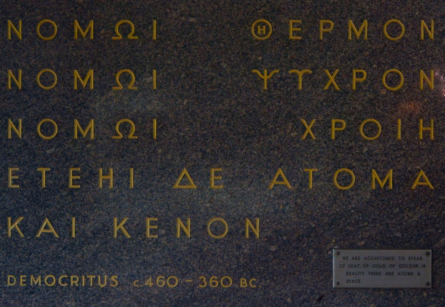
\includegraphics{Chapter_2/Figs ch2/democritus.png}
    \caption{An inscription from the pre-Socratic philosopher, Democritus, welcomes visitors at the entrance of the UWA Physics building. This quote from over two millennia ago stands as one of the earliest written recognition's of atoms as nature's foundational building blocks. It reads, “By convention sweet and by convention bitter, by convention hot, by convention cold, by convention color; but in reality atoms and void.” Not bad for a 2400-year-old perspective. However, hopefully by the end of this chapter you will agree that Democritus's 'atom' might find a more accurate representation in the concept of a 'field'.}
    \label{fig:democritus}
\end{figure}

\section{Special relativity}

We can build our field theory based on some simple axioms:
\begin{enumerate}
    \item The laws of physics are the same in all inertial frames of reference (Principle of relativity).
    \item The speed of light in a vacuum is the same for all observers, regardless of their state of motion or the state of motion of the source of light.
\end{enumerate}

These postulates were first introduced by Einstein when he noticed some inconsistencies between Galileo's principle of relativity, and Maxwell's equations.  Maxwell's which state that the speed of light is the same in all reference frames, but Gelileo's principle of relativity would imply that different observers will measure different speeds of light.

Following these postulates to their logical conclusion leads to famous phenomena, such as time dialtion and length contraction. We can encode all the information we know from special relativity by considering consequence of these postulates is the metric, which is an invariant in all reference frames.

\begin{equation}\label{eq:Flat spacetime metric}
    s^2 = - (t_1-t_2)^2 + (x_1-x_2)^2 + (y_1-y_2)^2 + (z_1-z_2)^2
\end{equation}

Notice that there is a negative in front of the time contribution, this means distance in spacetime is not the same as distance in a general Euclidean space, so our intuition about distance in space does not exactly carry over to spacetime. This leads to many of the non-intuitive concepts of special and general relativity. The reason the metric is chosen in this way, is because all observers will agree on these distances, no matter where observers are or how they are moving. In general relativity, the metric changes in the presence of masses, i.e. distances between points is no longer the flat space distance, and therefore, the straightest path between two points is no longer a straight line.

%%%%%%%%%%%%%%
\section{Special Relativity and the Metric}

Special relativity, developed by Albert Einstein in the early 20th century, revolutionized our understanding of space and time. Its theoretical foundation is built upon two simple, yet profound postulates: 

\begin{enumerate}
    \item The laws of physics are the same in all inertial frames of reference (Principle of relativity).
    \item The speed of light in a vacuum is the same for all observers, regardless of their state of motion or the state of motion of the source of light.
\end{enumerate}

These seemingly straightforward axioms have far-reaching implications for our understanding of the universe. They necessitate the unification of space and time into a four-dimensional spacetime, a framework within which events and interactions are described. 

One of the cornerstones of special relativity is the concept of Lorentz invariance, which states that the laws of physics are unchanged under Lorentz transformations. These transformations describe how measurements of space and time by two observers moving at a constant speed relative to each other are related.

Within this framework, the concept of the metric arises naturally. The metric, defined in the context of special relativity as the Minkowski metric, is a mathematical function that provides a measure of the interval - an invariant distance - between two events in spacetime. The metric is a fundamental aspect of the geometry of spacetime, and the invariance of this interval under Lorentz transformations is a reflection of the symmetries of spacetime under special relativity.

The notion of the metric and its properties are crucial when we extend our understanding from special to general relativity. In general relativity, the metric becomes a dynamic quantity that encodes the curvature of spacetime due to mass and energy. This curvature is what we perceive as gravity. Thus, the simple axioms of special relativity lay the foundation for the modern understanding of the universe at a fundamental level.


%%%%%%%%%%%%%


\section{Electromagnetism as a Field Theory}

Electromagnetism, the theory describing the interactions between charged particles, is a prime example of a field theory. This theory, encapsulated in Maxwell's equations, is formulated around the electric ($\mathbf{E}$) and magnetic ($\mathbf{B}$) fields. These fields are assigned a value at every point in space and time, and their dynamics are dictated by Maxwell's equations, which in Gaussian-cgs units \footnote{The choice to use Gaussian-cgs units eliminates the nonphysical factor $k=\frac{1}{4\pi \epsilon_0}$ from the electrostatic force law, leading to the more elegant expression $\Vec{F} = \frac{q_1 \cdot q_2}{r^2}$. This system uses the unit of charge called the electrostatic unit (esu), force in dyne, energy in ergs, among others - More details to be filled in later.}, are expressed as:

\begin{align}\label{eq:Maxwells}
    \nabla \cdot \mathbf{E} &= 4\pi\rho \\
    \nabla \times \mathbf{E} &= -\frac{1}{c} \frac{\partial \mathbf{B}}{\partial t}\label{eq:Maxwell grad E} \\
    \nabla \cdot \mathbf{B} &= 0 \\
    \nabla \times \mathbf{B} &= \frac{4\pi}{c} \mathbf{J} + \frac{1}{c} \frac{\partial \mathbf{E}}{\partial t}\label{eq:Maxwell Partial E}
\end{align}

Where $\rho$ is the charge density, $\mathbf{J}$ is the current density, and $c$ is the speed of light.

The field theory approach to electromagnetism further shines when we consider the principle of least action. We can derive the dynamics of the electric and magnetic fields from a simple Lagrangian density $\mathcal{L}$, which is a function of the fields and their derivatives. The choice of the Lagrangian is guided by the need to obtain Maxwell's equations as the equations of motion and the requirement of Lorentz invariance:

\begin{equation}
    \mathcal{L} = -\frac{1}{16\pi} F_{\mu \nu} F^{\mu \nu} - A_\mu J^\mu
\end{equation}

Where $F_{\mu \nu}$ is the electromagnetic field tensor and $A_\mu$ is the four-potential. The first term represents the kinetic energy of the electromagnetic field, and the second term represents the interaction of the field with matter. The Lagrangian is constructed to be Lorentz invariant, reflecting the fact that the laws of electromagnetism are the same in all inertial frames of reference.

Applying the Euler-Lagrange equations to this Lagrangian, we obtain Maxwell's equations. This demonstrates how field theory and the principle of least action can lead us to the laws governing electric and magnetic fields. These principles provide a unified description of electric and magnetic phenomena and form the basis for quantum electrodynamics, the quantum field theory of electromagnetic interactions.


%%%%%%%%%%%


\section{Magnetic Reconnection and Physicality of Fields}

Magnetic reconnection is a fundamental process in plasma physics that vividly illustrates the physicality of fields. In essence, magnetic reconnection is a phenomenon in which the magnetic topology is rearranged and magnetic energy is converted into kinetic and thermal energy of the plasma.

The process begins when two oppositely directed magnetic field lines come into contact. The field lines break and then reconnect with each other, forming a new set of field lines. This process changes the topology of the magnetic field and accelerates plasma particles, leading to phenomena such as solar flares and auroras.

\subsection{Alfven's theorem}

\begin{figure}
    \centering
    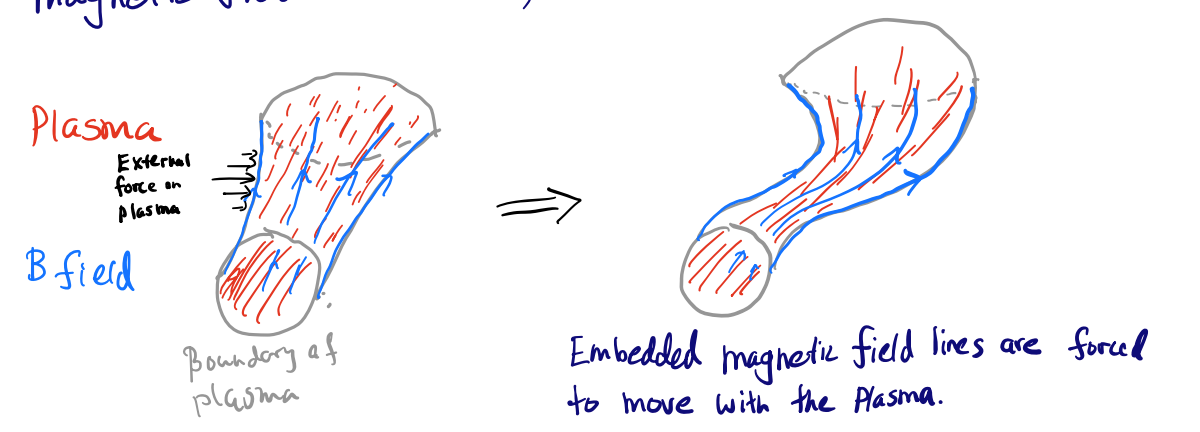
\includegraphics[width=\textwidth]{Chapter_2/Figs ch2/Alfven thm illustration 1.png}
    \caption{Illustration of Alfven's theorem - make better diagram}
    \label{fig:Alfven theorem}
\end{figure}

This reconnection process is a direct consequence of the properties of the magnetic field in a plasma. According to Alfvén's theorem, the magnetic field lines are "frozen" into the plasma under ideal conditions, meaning the magnetic field embedded within the plasma must move with the plasma - you can not move either the plasma or the magnetic field individually. This is demonstrated in figure \ref{fig:Alfven theorem}.

\begin{figure}
    \centering
    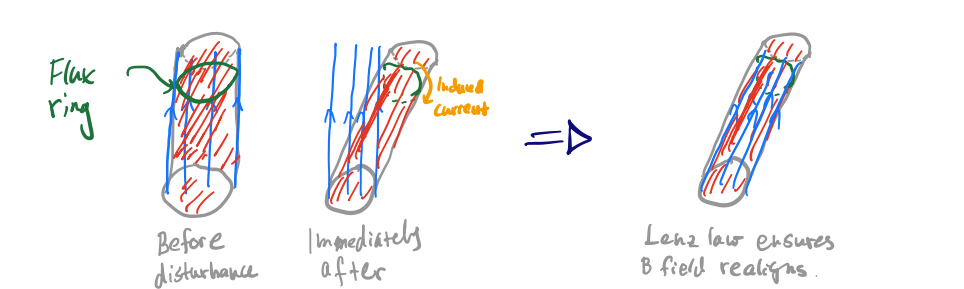
\includegraphics{Chapter_2/Figs ch2/Alfven theorem explanation 1.png}
    \caption{Explanation of Alfven's theorem through Lenz law. Obviously not an actual full proof.}
    \label{fig:Alfven through Lenz law}
\end{figure}

Alfvén's theorem can be intuitively understood by considering Lenz's law, which states that an induced electromotive force (or EMF) will always generate a current that creates a magnetic field opposing the change in the magnetic field. Consider a blob of Plasma, like that shown in figure \ref{fig:Alfven through Lenz law}. When we move a blob of plasma, the magnetic field lines embedded in it would initially remain stationary, becoming disconnected with the original configuration in the Plasma. However, this will result in a changing magnetic field through the Plasma, this change in the magnetic field will induce an electric field (Faraday's law of electromagnetic induction), which in turn drives a current. The induced current will then create a magnetic field that opposes the original change (assuming the idealized case of infinite conductivity of the Plasma - which is a good approximation in most cases).

As a result, any attempt to separate the plasma from the magnetic field lines is opposed by the induced magnetic field. Therefore, the magnetic field lines are effectively "frozen" into the plasma and move along with it, which is the essence of Alfvén's theorem.



% \begin{equation}
%     \frac{d \mathbf{B}}{dt} = \nabla \times (\mathbf{v} \times \mathbf{B})
% \end{equation}

% Where $\mathbf{B}$ is the magnetic field and $\mathbf{v}$ is the velocity of the plasma. This equation, derived from Maxwell's equations and the assumption of ideal magnetohydrodynamics (MHD), implies that if the plasma is moved, the field lines attached to it will also be moved.

% The proof that this result leads to Alfvens theorem is not obvious

\subsection{Magnetic reconnection}

\begin{figure}
    \centering
    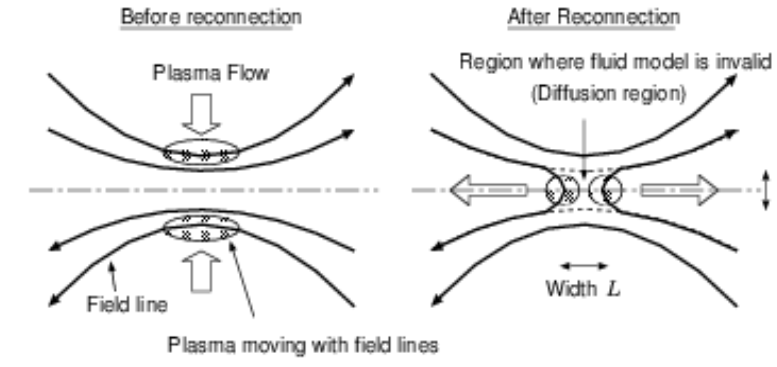
\includegraphics{Chapter_2/Figs ch2/reconnection illustration 1.png}
    \caption{Illustration of magnetic reconnection process. From \url{https://rnumata.org/research/recon}}
    \label{fig:reconnection illustration 1}
\end{figure}

To see how magnetic reconnection occurs, imagine two regions of Plasma next to one another, with each region having magnetic fields oriented in the opposite direction. Setting up a pressure gradient from each region towards the centre will lead each Plasma to move towards the centre, which by Alfven's theorem means the two magnetic fields will approach the centre - as illustrated on the left hand side of figure \ref{fig:reconnection illustration 1}. Due to the continuity of the magnetic field, the field lines must both vanish at this central point - which indeed does occur due to a process called magnetic diffusivity, a consequence of the fact that there are regions in a Plasma (called "current sheets") where conductivity is not infinite. This means there is a magnetic null point at the central region, which allows the magnetic field to reconnect into a new topology, by connecting with field lines on the opposite end of the boundary - as shown in the right hand side of figure \ref{fig:reconnection illustration 1}. By flux conservation, the inflowing Plasma is pushed outwards in the opposite direction, dragging the newly configured magnetic fields out with it. This results in a large release of energy, due to the energy stored within the magnetic field that vanished at the reconnection point.

This magnetic reconnection happens frequently in Astrophysical situations. For example, magnetic reconnection in the sun results in ejection of huge amounts of energy in the form of relativistic particles and Plasma, this is what is responsible for solar flares and coronal mass ejections.

\subsection{Physical nature of fields}

Alfvén's theorem and the concept of magnetic reconnection make it clear that fields are not just abstract mathematical constructs for calculations, but they have tangible physical effects. They store/release energy, %and respond to environmenntal changes as would a praticle

The magnetic field lines in a plasma are physical entities that affect and are affected by the motions of the plasma. As we will see in later sections, understanding the behavior of these field lines is crucial for understanding many phenomena in plasma physics and astrophysics. We will also come back to magnetic reconnection later on in this thesis, so stay tuned.


\section{General relativity}

\subsection{Additional postulates}

After Einstein discovered special relativity, he noticed it was limited. To go beyond special relativity, we need to add two more postulates:

\begin{enumerate}
    \item The principle of covariance.
    \item The equivalence principle.
\end{enumerate}

The theory of general relativity (GR) was developed by Albert Einstein to reconcile the laws of mechanics with the laws of the electromagnetic field. Special relativity, Einstein's previous formulation, was constrained to inertial frames and flat spacetime. To extend the theory to all coordinate systems—both inertial and non-inertial—Einstein added two more postulates: the principle of covariance and the equivalence principle.

The principle of covariance, also known as the principle of general relativity, asserts that the laws of physics must take the same mathematical form in all coordinate systems (i.e. we must write equations in tensor notation). This led to the concept of a four-dimensional spacetime, where the geometry can be curved by the presence of mass and energy.

The equivalence principle, on the other hand, states that locally the laws of physics reduce to that of special relativity.  Einstein famously came up with this principle while imagining a man falling off a building, and observing that in his perspective he is free of any forces. The principle also states that this man would would not be able to tell the difference between the acceleration he was experiencing due to gravity from what he would experience being uniformly accelerated through space by a jet pack (assuming of course that the man had no other form of sensation other then his acceleration, as if he was inside a dark chamber with no view of the world outside). This principle leads to the notion of a \textit{locally inertial reference frame}, a frame that follows the motion of a freely falling particle in a small region of spacetime. This is required because there is no such thing as a globally inertial reference frame in general relativity, since we can imagine a particle that begins at rest with respect to this global frame, but begins accelerating and hence begins to move according to this frame.

Since there is no global inertial reference frame in GR, we must define a new geometry for spacetime then the one described by $\eta_{\mu \nu}$ in special relativity - i.e. we need a spacetime that changes from point to point. From Einstein's equivalence principle, this geometry must be locally flat, i.e. for a given point in spacetime we can choose coordinates such that in a small enough region the spacetime can be described by the metric $\eta_{\mu \nu}$. A geometry that is locally flat is known as a \textit{manifold} - for example, the surface of the Earth is a manifold since from out in space it looks like a sphere, but to an ant - who can only observe a small chunk of the Earth at a time - it is flat. Einstein then postulated that gravity emerges as a result of the curvature of this spacetime - like how a ball rolled over the surface of a trampoline distorted by a large bowling ball in the centre will be deflected towards the balling ball - any particle in spacetime will be deflected in the direction of other massive objects. We will make this intuitive notion more precise in the following sections.

\subsection{Why general relativity is hard}
Recall that the electromagnetic field is sourced by the current four vector $J^\mu=\left(\rho, \Vec{j}\right)$ , produced by charged particles moving through space, leading to a field that can be described by another four vector $A^\mu=(\phi, \Vec{A})$. In general relativity, the source is now the energy-momentum/stress tensor $T_{\mu \nu}$, which contains information about particle momentum (described by a single four vector) as well as particle energy (described by another four vector) and hence is a rank two tensor. This results in a field that is also rank two, called the metric $g_{\mu \nu}$, which turns out to be a generalization of the space-time interval we found in special relativity. In fact, the spacetime metric $\eta_{\mu \nu}$ is the metric for flat spacetime, while in general $g_{\mu\nu}$ describes the distance between events in curved spacetime. $ds^2 = g_{\mu \nu} dx_\mu dx_\nu$ gives the infinitesimal displacement of two events in the spacetime described by the metric $g_{\mu \nu}$.

When we say space-time is curved, what we mean is that the coordinate system we use to describe events changes as we move between points in spacetime. When a light ray passes by the gravitational field of the sun, the mass-energy of the sun curves spacetime more strongly closer to its surface, meaning . This is very similar to how light rays travelling through a medium with a smoothly varying index of refraction will curve towards the side with the lower index of refraction, since light travels faster in a higher index of refraction - but now light (or anything with mass/energy) is bending towards in the direction of the decreasing metric.

So general relativity requires studying how fields change along space-time, with the coordinates describing the space-time also changing from point to point. This means our standard derivative from calculus is not going to cut it, we need to account for both the change in the field and the change in the coordinates. So to describe GR, we need tools from the mathematical subject called \textit{differential geometry}. 

\subsection{Differential geometry}

Consider a function $f$ defined on a curve $x^\mu(\lambda)$, then the ordinary derivative of f can be found by the chain rule
\begin{equation}
    \frac{df}{d\lambda} = \frac{\partial f}{\partial x^\mu} \frac{dx^\mu}{d\lambda}.
\end{equation}
We call $\frac{\partial f}{\partial x^\mu} := \partial_\mu f$ the gradient of f, this has a lower index and is called a contravariant derivative, because with a change of coordinates it transforms in the opposite way that a vector does. Indeed, using the chain rule we see that a change of coordinates $x^\alpha \rightarrow x^{\alpha'}(x^\alpha)$, then 
\begin{equation}
    \frac{\partial f}{\partial x^{\alpha '}} = \frac{\partial f}{\partial   x^\alpha} \frac{\partial x^\alpha}{\partial x^\alpha'}
    \implies
    \partial_{\alpha'} f = \partial_{\alpha} f \cdot \frac{\partial x^{\alpha}}{\partial x^{\alpha'}}
\end{equation}

While a vector $A^\mu$ transforms covariantly as 

\begin{equation}
    \frac{\partial A^\mu}{\partial x^{\nu'}} = \frac{\partial A^\mu}{\partial x^\alpha} \frac{\partial x^\rho}{\partial x^{\nu'}}.
\end{equation}

In general, a tensor ${T^{\alpha ... \beta}}_{\gamma ... \delta}$ of type (n, m) transforms with a change of coordinates according to the rule
\begin{equation}
    {T^{\alpha' ... \beta'}}_{\gamma' ... \delta'}=\frac{\partial x^{\alpha'}}{\partial x^\alpha} \cdot\cdot\cdot \frac{\partial x^{\beta'}}{\partial x^\beta}  \cdot \frac{\partial x^{\gamma}}{\partial x^\gamma'} \cdot\cdot\cdot \frac{\partial x^{\delta}}{\partial x^\delta'} \cdot {T^{\alpha ... \beta}}_{\gamma ... \delta}.
\end{equation}
However, the gradient of an arbitrary tensor is not itself a tensor, this is a problem as it violates the principle of covariance. This we need a new type of derivative, one that is covariant. In GR one of these derivatives is known as the \textit{covariant derivative}, which is built from the standard partial derivative, but contains a correction term such that the covariant derivative of a tensor is also a tensor. The covariant derivative is given by

\begin{equation}
    \nabla_\beta A^\alpha = \partial_\beta A^\alpha + \Gamma^{\alpha}_{\mu \beta} A^\mu
\end{equation}.
The coefficients $\Gamma^{\mu}_{\nu \sigma}$ are called the connection.  Einstein's principle of equivalence  demands the  connection be symmetric $\Gamma^{\alpha}_{\mu \beta} = \Gamma^{\alpha}_{\beta \mu}$ and metric compatible $\nabla_{\gamma} g_{\alpha \beta} = 0$, this allows us to uniquely define the metric according to the formula

\begin{equation}
    \Gamma^{\mu}_{\nu \sigma} = \frac{1}{2} g^{\alpha \mu} (\partial_{\nu}g_{\alpha \sigma}+\partial_{\sigma} g_{\nu \alpha} - \partial_{\alpha} g_{\nu \sigma}).
\label{eq:Christoffel symbol}
\end{equation}

These gamma coefficients are now called the \textit{Christoffel symbols}, they give the change in the tensor due to the change in the coordinates between points. A tensor field is said to be \textit{parallel transported}  along a curve $\gamma$ if its covariant derivative $\nabla_{\gamma} T^{\alpha ...}_{\beta ...} = 0$ vanishes. This intuitively means that the tensor remains parallel with the surface it is moving under - this allows us to compare two tensors located at different points in spacetime - which is not trivial in curved spacetime.

The paths followed by particles in general relativity correspond to shortest paths through (curved) space-time. These shortest paths are known as geodesics, and the formula for determining these paths is know as the geodesic equation

\begin{equation}
    \frac{d^2x^{\mu}}{d\tau^2} + \Gamma^{\mu}_{\nu \sigma} \frac{dx^{\nu}}{d\tau} \frac{dx^{\sigma}}{d\tau} = 0
\label{eq:Geodesic equation}
\end{equation}

This equation is derived by minimizing the action $S$ defined by

\newcommand{\Lagr}{\mathcal{L}}

\begin{equation}
    S = \int \mathcal{L}(x_\mu,\dot{x}_\mu) d\lambda = \int \frac{1}{2} g_{\mu \nu} \dot{x}^\mu \dot{x}^\nu d\lambda 
\label{eq:Invariant distance action}
\end{equation}

Using the Euler Lagrange equations

\begin{equation}
    \frac{d}{d\lambda} \frac{\partial \mathcal{L}}{\partial \dot{x_i}} - \frac{\partial \mathcal{L}}{\partial x_i} = 0
\label{eq:Euler-Lagrange equation}
\end{equation}

We can physically motivate this definition by considering that this is equivalent to extremizing the \textit{proper time} $\tau$ between two events\footnote{In special relativity, i.e. flat spacetime, time dilation means that the worldine of free particles moving between two events is the worldline of largest proper time between those events. General relativity says that this principle is extended to curved spacetime.}. The proper time is the time a clock carried by a particle will experience, while a distant observer (at a relative velocity and different gravitational field) will measure a different time between two events. So just find the extremal value of

\begin{equation}
    \tau_{AB} = \int \sqrt{- ds^2} = \int_0^1 \sqrt{-g_{\mu \nu}(x(\lambda))
    \frac{dx^\mu}{d\lambda} \frac{dx^\nu}{d\lambda}}d\lambda 
\label{eq:Proper time}
\end{equation}

Where $\lambda$ is the parametrization of the curve in space. Hence finding the maxima of equation \ref{eq:Proper time} is equivalent to finding the minima of the action given in equation (\ref{eq:Invariant distance action}), as required.

Another way to view equation (\ref{eq:Geodesic equation}) is as a path that is locally straight in curved spacetime. The particles four velocity

\begin{equation}\label{eq:Four velocity}
    \boldsymbol{u} := \frac{dx^\mu}{d\tau}
\end{equation}

Is always tangent to its path in space, the four velocity will therefore be straight if the four vector $\boldsymbol{u}$ does not change after an infinitesimal displacement.

\subsection{Einstein's field equation}
Doing the same thing we did with electromagnetism, we can derive the central equation of GR. We do this by noting that ...

Varying this action gives (derivation in appendix).

General relativity describes gravity as the result of mass curving spacetime, and the resulting curved spacetime causing particles to be deflected along there trajectory toward the mass - manifesting as the attractive Newtonian force we see in the classical world. So anything with mass, in fact anything with energy\footnote{Since by Einstein's mass energy equivalence, anything with energy has mass, and vice-versa.} causes spacetime to curve, as shown in the illustration of in figure \ref{fig:GR_analogy}. Then, any other object with energy within that spacetime will travel in straight lines across this spacetime, resulting in for example orbital motion. 

The way we precisely calculate how energy curves this spacetime, and how particles respond to this curvature, is with the \textit{Einstein field equations} (EFEs).

\begin{equation}
    G_{\mu \nu} + \Lambda g_{\mu \nu} = \kappa T_{\mu \nu}
\label{eq:EFE}
\end{equation}

Where 

\begin{itemize}
    \item $G_{\mu \nu}$ is the Einstein tensor, representing the curvature of space-time.
    
    \item $T_{\mu \nu}$ is the stress energy tensor, representing the density and flux of energy/momentum in space-time.
    
    \item $\Lambda$ is the cosmological constant, which gives rise to the accelerating expansion of the universe.
    
    \item $\kappa=\frac{8\pi G}{c^4}$ is a constant.
    
    \item $g_{\alpha \beta} = \boldsymbol{e}_\alpha \cdot \boldsymbol{e}_\beta$ is the metric tensor, given by the dot product of the basis vectors, and $g^{\alpha \beta}$ is the inverse metric tensor. The metric tensor allows for measurements of distance in space-time, and can be thought of as representing the gravitational field in general relativity.
 \end{itemize}


The Einstein tensor can be written as

\begin{equation}
    G_{\mu \nu } = R_{\mu \nu} - \frac{1}{2} R g_{\mu \nu}
\label{eq:Einstein tensor}
\end{equation}

Where the R tensor are contractions of the Ricci tensor defined by equation 

\begin{equation}
    R_{\sigma \mu \nu }^{\rho }=\partial_{\mu} \Gamma _{\nu \sigma }^{\rho }-\partial_\nu \Gamma _{\mu \sigma }^{\rho }+\Gamma _{\nu \sigma }^{\lambda } \Gamma _{\mu \lambda }^{\rho }-\Gamma _{\mu \sigma }^{\lambda } \Gamma _{\nu \lambda }^{\rho }
\label{eq:Riemann tesnor}
\end{equation}


\begin{itemize}
    \item $R_{\mu \nu} = R^{\alpha}_{\nu \alpha \beta}$ is the Ricci curvature tensor, which roughly represents how much the curved space-time deviates from flat space-time.
    \item R = $R^{\alpha}_{\alpha}$ is the Ricci scalar, the contraction of the Ricci tensor, a measure of curvature.
\end{itemize}

And gamma coefficients $\Gamma^{\mu}_{\nu \sigma}$ describes the Christoffel symbols (or affine connection), which itself is given by the formula

\begin{equation}
    \Gamma^{\mu}_{\nu \sigma} = \frac{1}{2} g^{\alpha \mu} (\partial_{\nu}g_{\alpha \sigma}+\partial_{\sigma} g_{\nu \alpha} - \partial_{\alpha} g_{\nu \sigma})
\label{eq:Christoffel symbol}
\end{equation}

These gamma coefficients represent how basis vectors change between points in space.

TODO: Go more into the intuition behind the terms in the EFEs.

\subsection{The weak field limit}

To elucidate the connection between the gravitational and electromagnetic field, we will approximate Einstein's field equations in the weak field limit. This introduces two new concepts, gravitoelectromagnetism, and gravitational waves.

TODO - Derivation of gravitomagnetic equations from weak field limit of general relativity.

\begin{align}\label{eq:Gravitomagnetic equations}
    \nabla \cdot \mathbf{E_g} &= - 4\pi G \rho_g \\
    \nabla \times \mathbf{E_g} &= - \frac{\partial \mathbf{B_g}}{\partial t}\label{eq:Gravitomag grad E} \\
    \nabla \cdot \mathbf{B_g} &= 0 \\
    \nabla \times \mathbf{B_g} &= - \frac{4\pi G}{c^2} \mathbf{J} + \frac{1}{c^2} \frac{\partial \mathbf{E_g}}{\partial t}\label{eq:Gravitomag Partial E}
\end{align}

Where $\mathbf{E_g}$ is the gravitoelectric field, $\mathbf{B_g}$ is the gravitomagnetic field, and $\rho_g$ is the mass density. Almost identical to Maxwell's equations in equations (\ref{eq:Maxwells}).

Imagine a charged sphere rotating about its axis. The rotating charges will form current loops, and hence an electric dipole will be generated. This electric dipole will exert effectively a magnetic force on an incoming charged particle, with the direction given by the right hand rule. Consider now, the analogous gravitational situation, i.e. a sphere of matter rotating about its axis. The rotation of the mass will result in a gravitomagnetic force acting on an incoming moving mass, this is known as the Lens-Thirring effect, and has been experimentally verified. This situation resembles very well the concept of frame dragging, a black hole rotating drags spacetime with it, and indeed the direction of the force from frame dragging can be found by using the right hand rule.

